In this section, the layer is described in terms of the hardware and software design. Specific implementation details, such as hardware components, programming languages, software dependencies, operating systems, etc. should be discussed. Any unnecessary items can be ommitted (for example, a pure software module without any specific hardware should not include a hardware subsection). The organization, titles, and content of the sections below can be modified as necessary for the project.

\subsection{Layer Hardware}
A description of any involved hardware components for the layer. For example, if each subsystem is a software process running on an embedded computer, discuss the specifics of that device here. Do not list a hardware component that only exists at the subsystem level (include it in the following sections).

\subsection{Layer Operating System}
A description of any operating systems required by the layer.

\subsection{Layer Software Dependencies}
A description of any software dependencies (libraries, frameworks, etc) required by the layer.

\subsection{Subsystem 1}
Descibe at a high level the purpose and basic design of this subsystem. Is it a piece of hardware, a class, a web service, or something else? Note that each of the subsystem items below are meant to be specific to that subystem and not a repeat of anything discussed above for the overall layer.

\begin{figure}[h!]
	\centering
 	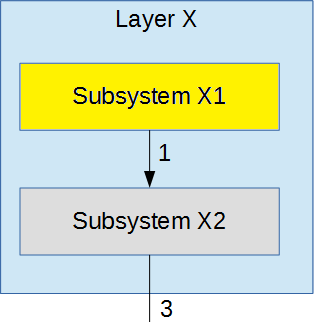
\includegraphics[width=0.60\textwidth]{images/subsystem}
 \caption{Example subsystem description diagram}
\end{figure}

\subsubsection{Subsystem Hardware}
A description of any involved hardware components for the subsystem.

\subsubsection{Subsystem Operating System}
A description of any operating systems required by the subsystem.

\subsubsection{Subsystem Software Dependencies}
A description of any software dependencies (libraries, frameworks, design software for mechanical parts or circuits, etc) required by the subsystem.

\subsubsection{Subsystem Programming Languages}
A description of any programming languages used by the subsystem.

\subsubsection{Subsystem Data Structures}
A description of any classes or other data structures that are worth discussing for the subsystem. For example, data being transmitted from a microcontroller to a PC via USB should be first be assembled into packets. What is the structure of the packets?

\subsubsection{Subsystem Data Processing}
A description of any algorithms or processing strategies that are worth discussing for the subsystem. If you are implementing a well-known algorithm, list it. If it is something unique to this project, discuss it in greater detail.


